\section{Methodology}
\label{s:methodology}

In this section, the implementation of the distributed file system will be
outlined. Firstly, the architecture of the file system will be described and how
the distributed part of the file system was simulated. The application 
interfaces will be described which serves as the file system operations that 
are supported. The communication interfaces will also be outlined.

\subsection{Architecture}
\label{s:architecture}

The distributed file system has a similar architecture to the Google File System.
\todo[inline]{Add reference to GFS.} There are two kinds of nodes in the system:
metadatanode and datanodes. There is a single metadatanode and multiple datanodes.

\begin{figure}[H]
    \centering
    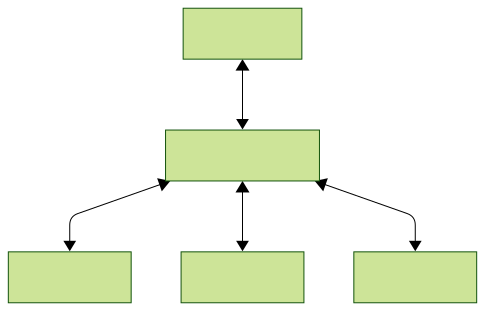
\includegraphics[width=\columnwidth]{images/architecture.png}
    \caption{Architecture Design for the Distributed File System. 
    The MetadataNode exposes the application API. The MetadataNode 
    and DataNodes communicate via the communication API.}
    \label{f:}
\end{figure}

\subsubsection{MetadataNode}
\label{s:metadatanode}
The single metadatanode is responsible for keeping track of all of the file
metadata and space for the file system. It has a few data structures that are
used to keep track of this information and ensure communication between itself
and the datanodes.

The first few data structures relate to the internal file system information. It
keeps track of the total number of blocks available given the capacity of the
file system. It keeps track of the available blocks with a bitmap.

The second type of data structures relate to the files metadata. It keeps track
of the number of files currently in the file system. Each file is structured with
its file name, and the number of blocks that it extends. Each file entry structure
keeps track of a file-to-block mapping, which helps us find the system block
given the file block (a file's block 0 might map to block 256 in the file system).

The third type of data structures are related to the datanode information and tracking.
The metadanode keeps track of how many datanodes have been created for this file
system, and keeps track of connections to these datanodes. 
It also keeps some additional data structures 

\subsection{DataNode}
\label{s:datanode}

\subsubsection{Application API}
\label{s:applicationapi}

The application API provides an interface for interacting with the metadatanode
in the distributed file system. It exposes functions for initializing and shutting
down the file system, creating, reading, writing, and managing file system and blocks.
The API is intended to be used by client applications that need to access or
manipulate file system data while abstracting the management.

The API can be categorized into three functional groups:
\begin{itemize}
    \item \textbf{Initialization and Cleanup}: Functions to start and stop the file
    system. Involves creating the various datanodes and connecting to them.
    \item \textbf{File Management:} Functions for creating, locating, truncating, reading,
    and writing to files.
    \item \textbf{Block-level Operations:} Functions for directly reading and writing
    individual file blocks.
\end{itemize}
 
\begin{lstlisting}
metadatanode_init(int num_dns, size_t capacity, const char *policy_name)
metadatanode_exit(int cleanup)

metadatanode_create_file(const char *filename, size_t file_size, int *fid)
metadatanode_find_file(const char *filename, int *fid)
metadatanode_truncate_file(int fid, size_t new_size)
metadatanode_read_file(int fid, void **buffer, size_t *file_size)
metadatanode_write_file(int fid, void *buffer, size_t buffer_size)

metadatanode_read_block(int fid, int file_index, void *buffer)
metadatanode_write_block(int fid, int file_index, void * buffer)
\end{lstlisting}

As mentioned previously, on the creation of a file, a file id is created.

\subsubsection{Communication API}
\label{s:communicationapi}

The communication API provides an interface for the communication between the
metadatanode and the datanodes in the distributed file system. It exposes
functions for each type of node to send commands, receive commands,
and responses to the commands.

\begin{lstlisting}
    md_send_command(int sock_fd, DNCommand cmd, void *payload, size_t payload_size)
    md_recv_response(int sock_fd, DNStatus *status, void **payload, size_t *payload_size)
    dn_recv_command(int sock_fd, DNCommand *cmd, void **payload, size_t *payload_size)
    dn_send_response(int sock_fd, DNStatus status, void *payload, size_t payload_size)
\end{lstlisting}

There are six types of commands that the metadatanode can use to communicate with
the datanode \texttt{DN\_INIT}, \texttt{DN\_ALLOC\_BLOCK}, 
\texttt{DN\_FREE\_BLOCK}, \texttt{DN\_READ\_BLOCK}, \texttt{DN\_WRITE\_BLOCK}, 
\texttt{DN\_EXIT}. Each command is used alongside a buffer which sends the appropriate
information for that command. For example, \texttt{DN\_READ\_BLOCK} requires the
block index to be read.

\subsection{Policies}
\label{s:policies}

\subsubsection{Random}

\subsubsection{Sequential}

\subsubsection{Round Robin}

\subsubsection{Least Loaded}

\subsubsection{File Aware}

\subsection{Workloads}
\label{s:workloads}
